\documentclass{beamer}
\usepackage[portuguese]{babel}
\usetheme{uic}
\usepackage{amsfonts,amsmath,oldgerm,algorithmic,algorithm}
\usepackage[font=small,labelfont=bf]{caption} % Required for specifying captions to tables and figures

\newcommand{\hrefcol}[2]{\textcolor{uihteal}{\href{#1}{#2}}}
\newcommand{\testcolor}[1]{\colorbox{#1}{\textcolor{#1}{test}}~\texttt{#1}}

% Please see Section 18.1 of Beamer User Guide for all the options \usefonttheme provides
\usefonttheme[onlymath]{serif}
% \usefonttheme{serif} % use this if you would like Serif font throughout (and not just for math)

\title{Apresentação de Artigo}
\titlebackground{images/tema_fundo_6.png}
% an asterisk will split the background:
% \titlebackground*{images/uic_seo.jpg}
\subtitle{De Autores do artigo}

\author{\href{mailto:augusto.adamns@ufpr.br}{Augusto Mathias Adams}}
\date{\today}

\begin{document}
\maketitle

% default is no footline, but page numbers are incredibly useful for the audience to ask questions later
\footlinecolor{uicblue}

\begin{frame}{Beamer for UIC presentations}
If you would like \LaTeX in your presentation, Beamer is a great way to go!
\begin{itemize}
\item Beamer has a detailed
\hrefcol{https://www.ctan.org/tex-archive/macros/latex/contrib/beamer/doc/beameruserguide.pdf}{user
 manual}, but we will go over the most common features.
\item The most common of all slide types involve bulleted points, like these.
\item Regular \LaTeX commands will help you type math, as below.
\begin{equation*}
\mathcal{L} (\theta) = \log \sum_{k=1}^{\lvert Z \rvert} Q(z_k \mid y) \frac{P( z_k,  y \mid \theta)}{Q(z_k \mid y)} \geq \sum_{k=1}^{\lvert Z \rvert} Q(z_k \mid y) \log \frac{P( z_k,  y \mid \theta)}{Q(z_k \mid y)}
\end{equation*}
\end{itemize}
\end{frame}


\begin{chapter}[images/bg_1.png]{uicblue}{Slide Layouts}
\textit{An overview of some different slide types you can have.}
\end{chapter}


\begin{frame}[fragile]{More with bullet points}
\framesubtitle{Unrolling}
\begin{itemize}[<+->]
\item You could also unroll the slides in a sequence.
\item Just added \verb|[<+->]| option to \verb|\begin{itemize}| in this frame.
\item P.S. If you end up using verbatim text (i.e. \verb|\verb| command) as I did to typeset the bullet point above, make sure to add \verb|[fragile]| option to your frame :)
\end{itemize}
\end{frame}


\begin{frame}[fragile]{More with bullet points}
\framesubtitle{Global alerts}
Sequential slide unrolling can be further enhanced using alerts.
\begin{itemize}[<alert@2>]
\item We will shortly show what they are.
\item<2- | alert@2> This is what they are :)
\end{itemize}
\end{frame}


\begin{frame}[fragile]{More with bullet points}
\framesubtitle{Local alerts}
Alerts can also be localized.
\begin{itemize}
\item The \verb|\alert{}| command provides this functionality.
\item Like \alert<2>{this}.
\item You may as well choose the highlighting to stick.
    \begin{itemize}
    \item Previous one did not, but \alert<3->{this one} will.
    \end{itemize}
\item Another common slide type involves columns and/or images.
    \begin{itemize}
    \item We show them in the \alert<4>{next slides}.
    \end{itemize}
\end{itemize}
\end{frame}


\begin{frame}[fragile]{Images and columns}
\begin{columns}
\begin{column}{0.7\textwidth}
Adding images works like in normal \LaTeX:
\begin{block}{Code for Adding Images}
\begin{verbatim}
\usepackage{graphicx}
% ...
\includegraphics[width=\textwidth]
{images/uic_quad.pdf}
\end{verbatim}
\end{block}
This slide layout was achieved using the \verb|columns| feature. The number and widths of the columns is totally user preference. Another columns example follows on the next slide.
\end{column}
\begin{column}{0.3\textwidth}
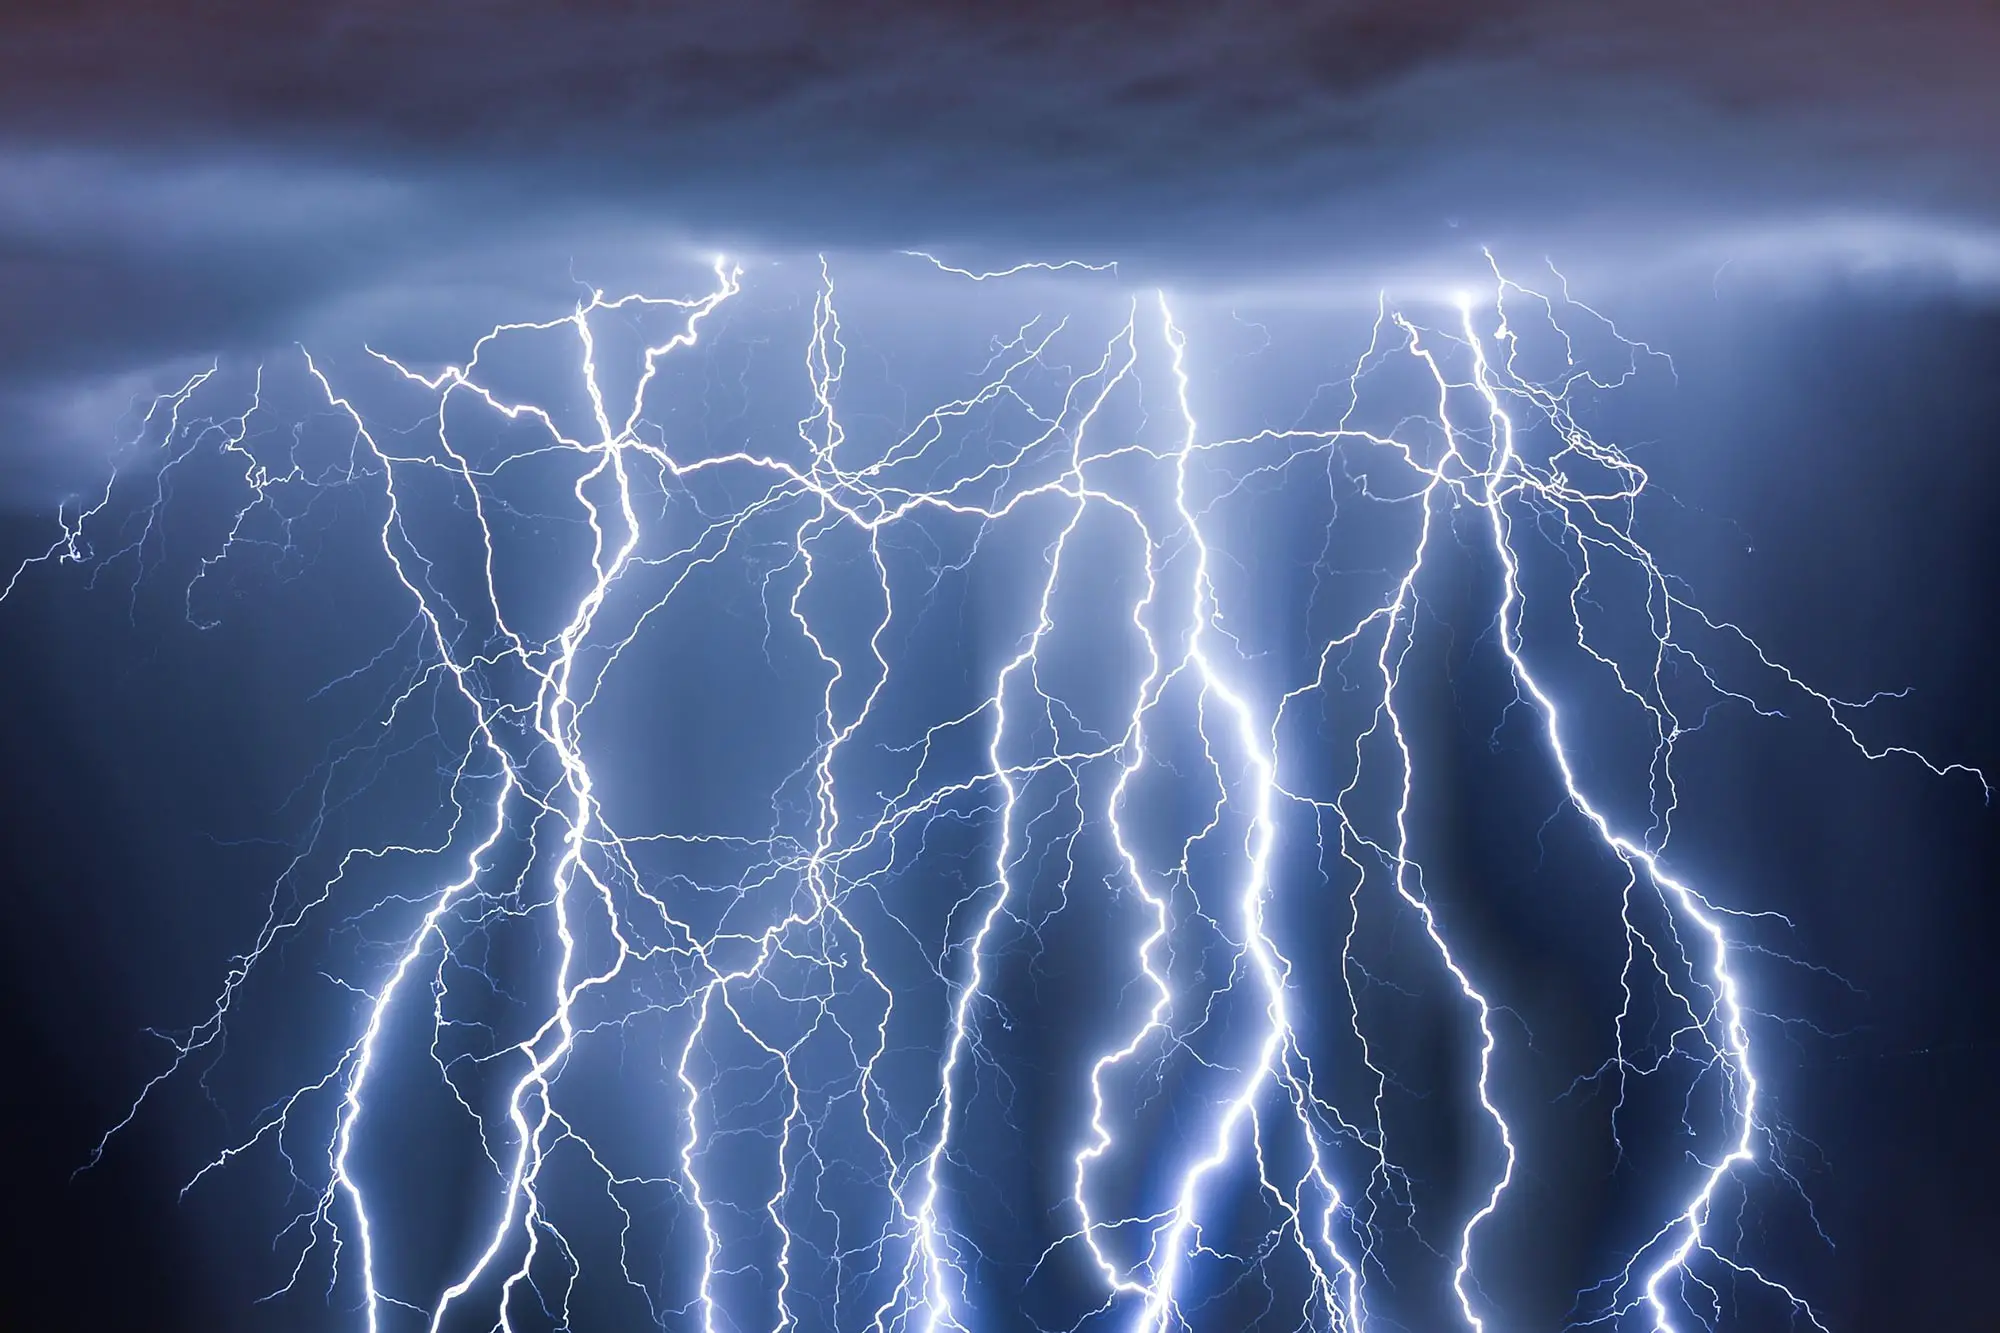
\includegraphics[width=\textwidth]
{images/bg_3.png}
\end{column}
\end{columns}
\end{frame}


\begin{frame}{Another images/columns example}
\begin{columns}
\begin{column}{0.35\textwidth}
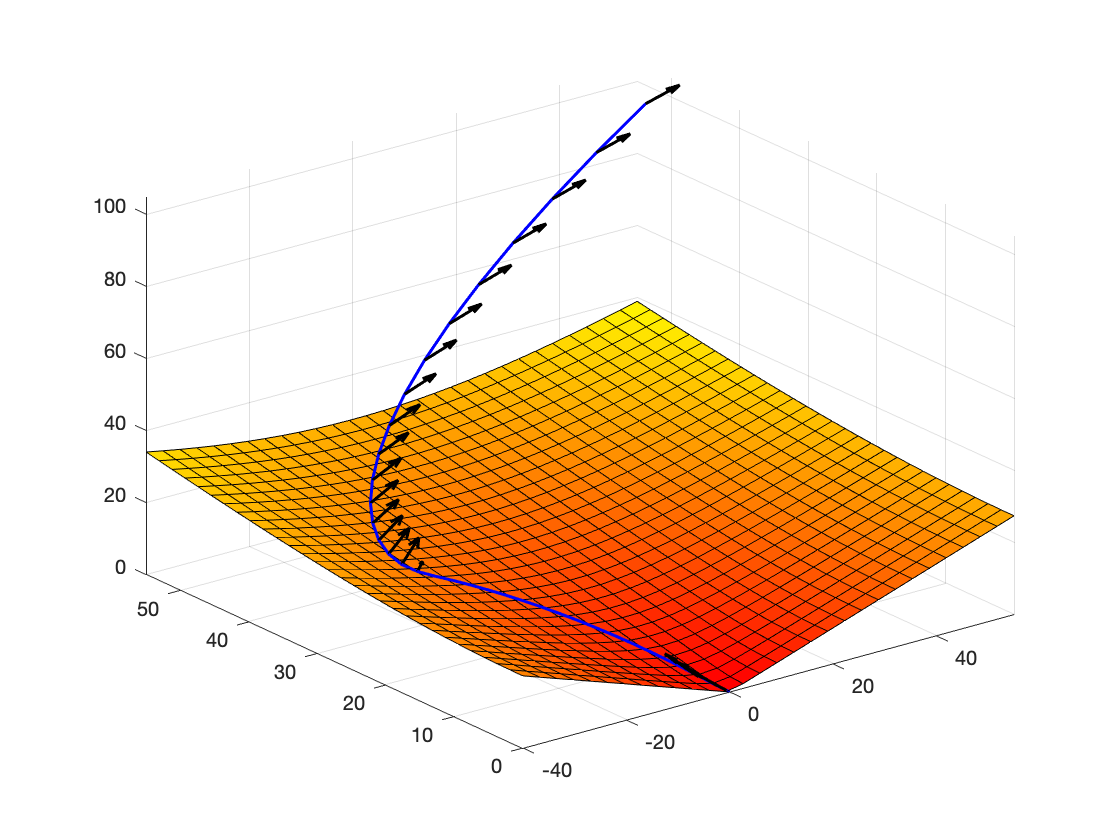
\includegraphics[width=\textwidth]{plots/min_fuel.png}
\captionof{figure}{Minimum fuel trajectory}
\end{column}
\begin{column}{0.3\textwidth}
\textbf{Left:} Solving for optimal fuel consumption \textbf{Right:} Solving for optimal time taken
\end{column}
\begin{column}{0.35\textwidth}
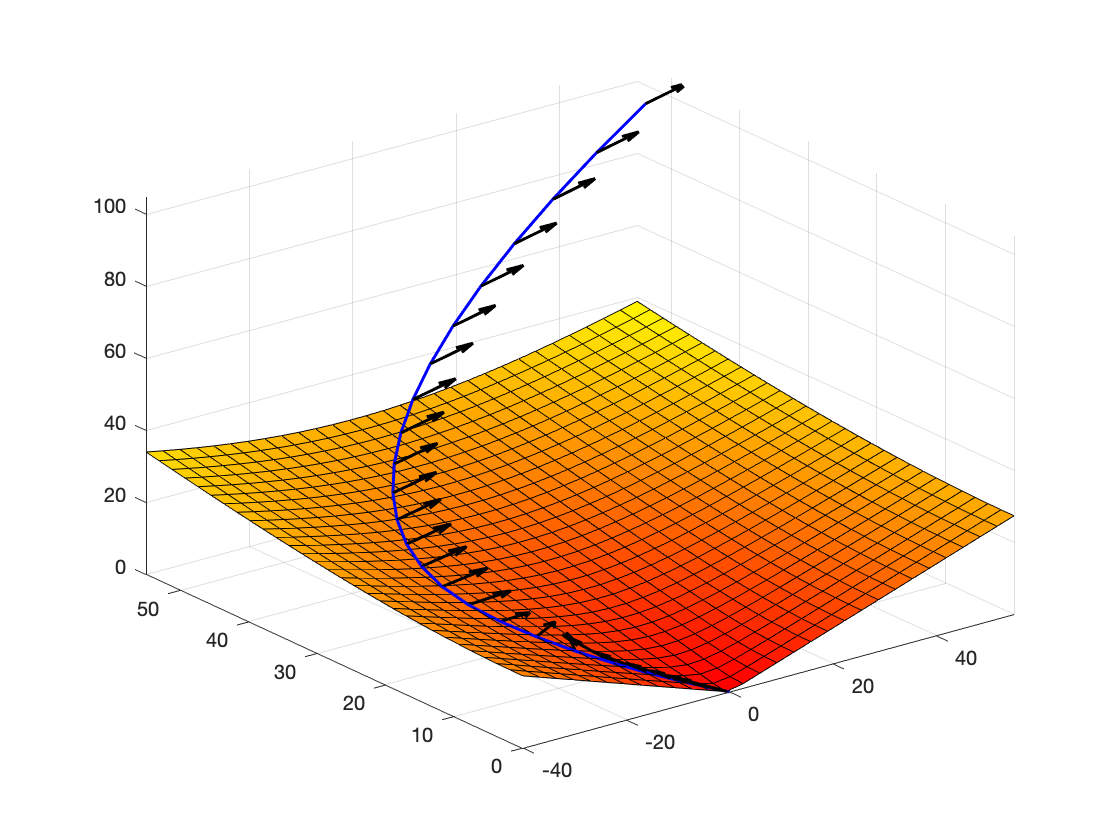
\includegraphics[width=\textwidth]{plots/min_time.png}
\captionof{figure}{Minimum time trajectory}
\end{column}
\end{columns}
\end{frame}


\begin{frame}[fragile]{Blocks for theorems}
Blocks are a great UI element and can be used for typesetting theorems.
\begin{block}{Theorem}
If $\mid \mathcal{H} \mid < \infty$, then $\mathcal{H}$ is PAC Learnable.
\end{block}
\end{frame}


\begin{frame}[fragile]{Blocks for partitioning}
Blocks are also a great way to partition your slide. They can be combined with columns, as shown here.
\begin{columns}
\begin{column}{0.3\textwidth}
\begin{block}{Standard Blocks}
For the light theme, their color matches the footline. We will discuss light and dark themes soon.
\begin{verbatim}
\begin{block}{title}
content...
\end{block}
\end{verbatim}
\end{block}
\end{column}
\begin{column}{0.7\textwidth}
\begin{colorblock}[black]{uihteal}{Color Blocks}
Similar to the ones on the left, but you pick the color. Text will be white by 
default, but you may set it with an optional argument.
\small
\begin{verbatim}
\begin{colorblock}[black]{uihteal}{title}
content...
\end{colorblock}
\end{verbatim}
\end{colorblock}
\end{column}
\end{columns}
\end{frame}


\begin{sidepic}{images/bg_1.png}{Side-Picture Slides}
Just another another layout you may want to use.
\begin{itemize}
\item These type of slides are created using \texttt{$\backslash$begin\{sidepic\}\{<image>\}\{<title>\}}
\item Otherwise, \texttt{sidepic} works just like \texttt{frame}
\end{itemize}
\end{sidepic}


\renewcommand{\algorithmicrequire}{\textbf{Input:}}
\renewcommand{\algorithmicensure}{\textbf{Output:}}
\newcommand*\CALL[2]{\textsc{#1}(#2)}
% \newcommand*\ANNOTATE[1]{\hfill\{#1\}}%
% \newcommand*\ANNOTATE[1]{\hskip3em$\rightarrow$ #1}
\newcommand*\ANNOTATE[1]{\hfill\(\triangleright\) #1}%

\footlinecolor{}

\begin{frame}[fragile]{Pseudocode Example}
\begin{algorithm}[H]
\fontsize{8}{1}\selectfont
\caption{Running EM using the joint PMFs, $P$, $Q$, $\hat P$}
\begin{algorithmic}
\REQUIRE A belief network $\mathcal{G}$ and dataset $ \mathcal{D}$
\ENSURE ML estimate of network parameter matrix $\hat P$
\STATE $\hat P \gets$ \CALL{RandomPMF}{}
\STATE $\text{LogLikelihood} \gets \text{empty list}$
\STATE $t \gets 0$
\REPEAT
    \STATE $\text{CurrentLogLikelihood} \gets 0$
    \STATE $Q \gets 0$
    \FOR{$d \in \mathcal{D}$}
        \STATE $\hat P(z_d \mid y_d) \gets \hat P(z_d, y_d) \delta(y_d)$
        \STATE $\text{CurrentLogLikelihood} \gets \text{CurrentLogLikelihood}$ + \CALL{Sum}{$\hat P(z_d \mid y_d)$}
        \STATE $Q \gets Q + \hat P(z_d \mid y_d) \times \delta(y_d)$ \ANNOTATE{E-step}
    \ENDFOR
    \STATE $\text{LogLikelihood}[t] = \text{CurrentLogLikelihood}$
    \STATE $\hat P \gets$ \CALL{Normalize}{$Q$} \ANNOTATE{M-step}
    \STATE $t \gets t + 1$
\UNTIL{convergence}
\RETURN $\hat P$
\end{algorithmic}
\end{algorithm}
\end{frame}


\footlinecolor{uicblue}

\begin{chapter}[images/bg_2.png]{uicblue}{Personalization}
\textit{Themes, fonts and colors}
\end{chapter}


\begin{frame}[fragile]{Let's talk themes}
Three fundamental features greatly affect the look and feel of your slides. Two of them can be controlled with the \verb|\themecolor| command.
\begin{itemize}
\item The background color.
\begin{itemize}
    \item The default is \verb|light| theme, which has a light background, which we are currently using.
\end{itemize}
\item The foreground color.
\begin{itemize}
    \item The \verb|light| theme has a \verb|dark| foreground (i.e. text color) and vice versa.
\end{itemize}
\item The third, the footer color can be set using \verb|\footlinecolor| command.
\begin{itemize}
    \item We are currently using \testcolor{uicblue} color for our footer.
    \item The default is no footline, but I believe page numbers are incredibly helpful for your audience to ask questions later.
\end{itemize}
\end{itemize}
\end{frame}


\themecolor{dark}
\usebeamercolor[fg]{normal text}
\footlinecolor{uicred}
\begin{frame}[fragile]{Let's talk themes}
\begin{itemize}
\item I just called \verb|\themecolor{dark}| before \verb|\begin{frame}| for this slide.
\begin{itemize}
    \item Ideally you should set the theme globally in the preamble (i.e. before \verb|\begin{document}|). Default is light.
    \item If you switch the theme from light to dark or vice versa in the middle of the presentation (like we just did), you \textbf{may} have to follow up with \verb|\usebeamercolor[fg]{normal text}| as well, as we did for this slide, otherwise the foreground color might not be automatically updated.
\end{itemize}
\item You can also change the footer color with \verb|\footlinecolor{color}|, as we did for this slide.
\item All the changes we talked about here happen for the current \textbf{as well as subsequent} frames.
\begin{itemize}
    \item I will manually revert all the changes for the next slide.
\end{itemize}
\end{itemize}
\end{frame}


\themecolor{light}
\usebeamercolor[fg]{normal text}
\footlinecolor{uicblue}


\begin{frame}[fragile]{Fonts}
\begin{itemize}
\item Fonts play a huge role in the look and feel of your presentation
  \begin{itemize}
  \item Their main purpose however, is clarity!
  \end{itemize}
\item \textrm{Serif} vs \textsf{Sans-Serif} fonts
  \begin{itemize}
  \item \hrefcol{https://www.adobe.com/creativecloud/design/discover/serif-vs-sans-serif.html}{This} is a good read on when to use which.
  \item \textbf{Open Sans} and \textbf{IBM Plex Serif} have been provided with this template.
  \item To conveniently switch from Open Sans to IBM Plex Serif, please use \verb|\usefonttheme{serif}| in the preamble.
    \begin{itemize}
    \item IBM Plex Serif is not available on \verb|pdfLaTeX|, so Caladea will be used instead.
    \end{itemize}
  \end{itemize}
\item The fonts provided in the \verb|fonts| folder (or your own fonts) can only be used with \verb|XeLaTeX|.
    \begin{itemize}
    \item The Overleaf version of this template uses \verb|XeLaTeX| by default.
    \item Next few slides talk about font formats and how they work with different compilers.
    \end{itemize}
\end{itemize}
\end{frame}


\begin{frame}[fragile]{Font formats over time}
Here are the \textbf{old} formats (still used in the LaTeX ecosystem):

\begin{itemize}
\item \emph{PostScript Type 1} format developed by Adobe in 1980s
\begin{itemize}
    \item Support officially ended by Adobe in January 2023
\end{itemize}
\item \emph{TrueType format} (\verb|.ttf|) developed by Apple, also in 1980s, licensed to Microsoft
\end{itemize}

The \textbf{new} font formats are \emph{OpenType}, developed jointly by Microsoft and Adobe in the 1990s as an extension of Apple's TrueType font format. \emph{OpenType} fonts are either

\begin{itemize}
\item \emph{PostScript flavor OpenType} (\verb|.otf|) that supercedes Adobe's PostScript Type 1
\item \emph{TrueType flavor OpenType} (also \verb|.ttf|!) that supercedes Apple's TrueType
    \begin{itemize}
    \item Distinguishing them from the old TrueType format is therefore non trivial.
    \end{itemize}
\end{itemize}
\end{frame}


\begin{frame}[fragile]{Font formats compatibility}
The new \emph{OpenType} fonts have several new features over the old formats. They are however, supported natively only by \verb|XeLaTeX| and \verb|LuaLaTeX| compilers. The most popular \verb|pdfLaTeX| compiler has limited support for them:
\begin{itemize}
\item \emph{OpenType} fonts are not \verb|pdfLaTeX|-ready by default.
\item They require the production of TeX font metrics and other ancillary files in order to be used with LaTeX.
\item The production of these files is not easy for the average user.
\end{itemize}
Consequently, if using \verb|pdfLaTeX|, the most convenient option is to restrict yourself to the fonts packages available at the \hrefcol{https://tug.org/FontCatalogue/}{LaTeX Font Catalogue}, which are already \verb|pdfLaTeX|-ready.
\end{frame}


\begin{frame}[fragile]{Font formats compatibility}
If you want to use fonts beyond those in the \hrefcol{https://tug.org/FontCatalogue/}{LaTeX Font Catalogue} (for example, fonts from Google Fonts), the recommended approach is to use \verb|XeLaTeX|.
\begin{itemize}
\item \verb|XeLaTeX| is set as the default compiler on the Overleaf version of this template.
\item The fonts included in the \verb|fonts| folder are \emph{TrueType flavor OpenType} fonts.
\item You can still use \verb|pdfLaTeX|, except that the included fonts will not be applied.
\end{itemize}
UIC signature font is Theinhardt, also available as \emph{OpenType}.
\begin{itemize}
\item Due to licensing issues, I cannot distribute Theinhardt with this template.
\item A licensed copy of Theinhardt can be obtained by UIC students and faculty \hrefcol{https://marketing.uic.edu/marketing-toolbox/uic-fonts/}{here}.
\end{itemize}
\end{frame}


\begin{frame}[fragile]{Text color}
\begin{itemize}
\item Font color can be set with the \verb|\textcolor{<color name>}{text}| command.
\item The colors are defined in the \texttt{uiccolor} package, in accordance with the \hrefcol{https://marketing.uic.edu/marketing-toolbox/university-style-guide/visual-elements/}{UIC Visual Elements guide}:
  \begin{itemize}
  \item UIC's primary colors are Navy Pier Blue (\testcolor{uicblue}) and Fire Engine Red (\testcolor{uicred}).
  \item UIC's secondary colors are Chicago Blue (\testcolor{chicagoblue}), UI Health Teal (\testcolor{uihteal}) and Champions Gold (\testcolor{championsgold}).
  \item UIC's neutral colors are Expo White (\testcolor{expowhite}) and Steel Gray (\testcolor{steelgray} or \testcolor{steelgrey}).
  \end{itemize}
\item A \emph{simpler alternative} to font colors is often just \verb|\emph{}|.
\end{itemize}
\end{frame}


\begin{frame}[fragile]{Chapter slides}
\begin{itemize}
\item Allow you to partition your presentation into multiple chapters
\item Also \verb|frame|s, but with a few more options
\item Created with \verb|\begin{chapter}[<image>]{<color>}{<title>}|
  \begin{itemize}
  \item Image is optional, color and title are mandatory.
  \end{itemize}
\item Multiple background images have been provided in this template which may be used for chapter slides:
  \begin{itemize}
  \item Some campus photos that I have taken over the years and;
  \item some departmental logos.
  \item Let's look at a few examples!
  \end{itemize}
\end{itemize}
\end{frame}


\begin{chapter}[images/bg_3.png]{uicblue}{Title goes here}
\textit{Subtitle goes here}
\end{chapter}

\begin{chapter}[images/tema_fundo_2.png]{uicblue}{Title goes here}
\textit{Subtitle goes here}
\end{chapter}

\themecolor{lightnologo}
% these backgrounds already have the UIC circular logo, so we temporarily change the theme to lightnologo
\begin{chapter}[images/tema_fundo_3.png]{uicblue}{Title goes here}
\textit{Subtitle goes here}
\end{chapter}

\begin{chapter}[images/tema_fundo_4.png]{uicred}{Title goes here}
\textit{Subtitle goes here}
\end{chapter}

\begin{chapter}[images/tema_fundo_5.png]{steelgray}{Title goes here}
\textit{Subtitle goes here}
\end{chapter}
\themecolor{light}

\begin{frame}[fragile]{Other departments}
\begin{itemize}
\item Download your logo from \hrefcol{https://marketing.uic.edu/marketing-toolbox/university-style-guide/university-marks-logos/}{here}.
    \begin{itemize}
    \item What you need is ``departmental lockup in SVG format and inverted RGB color".
    \end{itemize}
\item Manually overlay it on a static color background using an SVG editor.
    \begin{itemize}
    \item You can look at \verb|uiccolor.sty| file for the numerical value of the UIC background colors.
    \end{itemize}
\item Make sure the overlay is exported in at least 1600 x 1200 resolution in PNG format (you will need to upscale your SVG overlay).
    \begin{itemize}
    \item LaTeX cannot natively handle SVG images (and PNG images, if not sufficiently large, will pixelate in the presentation).
    \end{itemize}
\end{itemize}
\end{frame}


\begin{frame}[fragile]{Good luck with your presentation!}
\begin{itemize}
\item This template is hosted on GitHub
    \begin{itemize}
    \item  \verb|https://github.com/usamamuneeb/uic-beamer-template|
    \end{itemize}
\item  I would appreciate contributions of all sorts (pull requests, identifying issues, etc).
\item  If you have any suggestions,
\hrefcol{mailto:umunee2@uic.edu}{send them to me!}
\end{itemize}
\end{frame}


\backmatter
\end{document}
